%\chapter{Modelling Phonemic Streams using Transformer Language Models}\label{chapter:modelling}
\chapter{Establishing phoneme-based LM pre-training}\label{chapter:modelling}
%\chapter{Pre-training LM with phoneme-based input representations}\label{chapter:modelling}

Language models are typically trained on large corpora of text in their default orthographic form. However, this is not the only option; representing data as streams of phonemes can offer unique advantages, including deeper insights into phonological language acquisition, improved performance on sound-based tasks, and a better understanding of the generalisability of LMs. Despite the advantages of training language models with phonemes, it remains to be established whether modern LM architectures encode grammatical knowledge and succeed at language understanding tasks when trained with a phoneme-based input representation. The challenge lies in evaluating the impact of phoneme-based training, given benchmarks are also largely orthographic. 

%Evaluating the impact of phoneme-based training is a challenge for two reasons. First, training and evaluation data need to be provided to a model in both a phonemic and graphemic representation. Second, it is non-trivial to select the transformations to convert orthographic text into phonemic representations and to evaluate how these individually affect a model's performance across a wide variety of benchmarks. 

%We then identify three key transformations which enable us to map from the written representation typically used to train language models to the phonemic representation often used in analytical studies (see \cref{fix:14-example}). Finally, we conduct a careful ablation of the three transformations: we train a language model on the same corpus of 100 million words with all combinations of the three transformations ($2^3$ configurations), evaluating the model's grammatical capabilities and its resulting performance on downstream language understanding tasks. 

This chapter thoroughly explores the phoneme-based training using two targeted experiments. First, the BabyLM pre-training dataset and evaluation benchmarks (introduced in \cref{sec:12-plausiblepretraining}) are used as a framework for training and evaluating BabyLMs with different input representations. By using \gpp, the data can be converted to phonemes, allowing for parallel training to establish the difference between the orthographic and phonemic modalities. Additionally, three key transformations are identified that separate standard subword-based input representations from the phoneme-based input representation, facilitating an ablation study of the effect of each transformation.

% We run a careful ablation of the effects of each of these transformation in isolation and combination. 

Secondly, in order to establish the size requirements of phoneme LMs, a suite of BabyLMs across parameter scales are trained on differently-sized subsets of the EnglishNA section of \ipachildes. This experiment provides the ideal parameters to use for training a phoneme LM on a dataset of a particular size, supporting the experiments conducted in \cref{chapter:phonology}.

% \paragraph{Analytical:} A phoneme-based representation is useful when using language models to study the distributional properties of phonemes \citep{mayer-2020-phonology-distribution} and phonological systems of languages more broadly \citep{eden-2018-phonological-distance}. Many language acquisition studies prefer using phonemes as a representation that more closely represents the human learning environment, which facilitates statistical learning experiments ranging from word segmentation \citep{Coltekin2017}, to past-tense formation \citep{kirov-2018-recurrent}, and broader lexico-syntactic knowledge \citep{lavechin}.

% \paragraph{Practical:} IPA-encoded text has been found to be beneficial for a variety of NLP tasks including lyric generation \citep{ding-2024-songcomposer}, text-to-speech \citep{sundararaman-2021-phonemebert, li-2023-phoneme-level-bert} and low-resource language modeling \citep{leong-whitenack-2022-phone}. Phonemes also benefit multi-lingual language modeling by establishing a universal representation shared between languages \citep{feng-2023-language-universal-phonetic, zhu-etal-2024-taste}. 

%We find that large language models are powerful statistical learners capable of learning grammar from a phonemic input representation. Although we observe a decrease in performance on some tasks, the degradation is not as substantial as has been anecdotally suggested by previous studies. Our ablation studies indicate that the impact of each transformation that we use to convert orthographic text to continuous phoneme streams depends on the downstream task; tasks in the BLiMP Supplement set are particularly sensitive to the use of phonemes, while those in GLUE are sensitive to character tokenization. A deeper analysis into these ablations reveals that many evaluation instances rely on information only present in written text (such as punctuation). Finally, we take advantage of the fact that we train models using phonemic streams and evaluate our models for phonological knowledge using the BabySLM benchmark. Our models achieve the best scores on this benchmark to date.%, suggesting that these models have many unexplored benefits. 

%Finally, because the models we train accept phonetic inputs we train the language models usrepresentation can be evaluated for phonological knowledge - we do so and we achieve the best scores on the BabySLM corpus to date. Our novel use of the byte-pair encoding (BPE) algorithm on text with spaces removed may also lead to interesting acquisition studies relating to word segmentation and lexicon learning. 

% We discuss the limitations of our transcription method and discuss the use of raw audio as an alternative input representation. Finally, we present the advantages of this input representation for multi-lingual and low-resource applications and encourage further work in phoneme-based language modeling. 


\section{Input representation transformations}

Whereas the typical input representation used in LMs consists of orthographic subwords with marked word boundaries, the phoneme-based input representation uses the phonemic modality, with phoneme-level tokenisation and no marked word boundaries. These were introduced formally in \cref{sec:12-subword} and \cref{sec:12-phonemic}, respectively. Here, three key transformations are identified that convert the subword-based representation to the phoneme-based representation:

\begin{itemize}
\setlength\itemsep{0.1em}
    \item \characterhighlight{Character tokenisation} Treating each phoneme or grapheme as a token, rather than using subwords.
    \item \spacehighlight{Word boundary removal} Removing whitespace or other word boundary cues from the input.
    \item \phonemehighlight{Phonemic transcription} Converting words to a phonemic representation. 
\end{itemize}

Each transformation can be made independently or in combination, as illustrated in \cref{fig:14-example}. Training LMs with each of the eight possible combinations allows for an ablation study, identifying the impact of each transformation individually. %Certain combinations have also rarely been considered; such as learning subword units from text stripped of word boundaries, or adding word boundaries to phoneme-level token sequences. 

\begin{figure}[t]
    \centering
    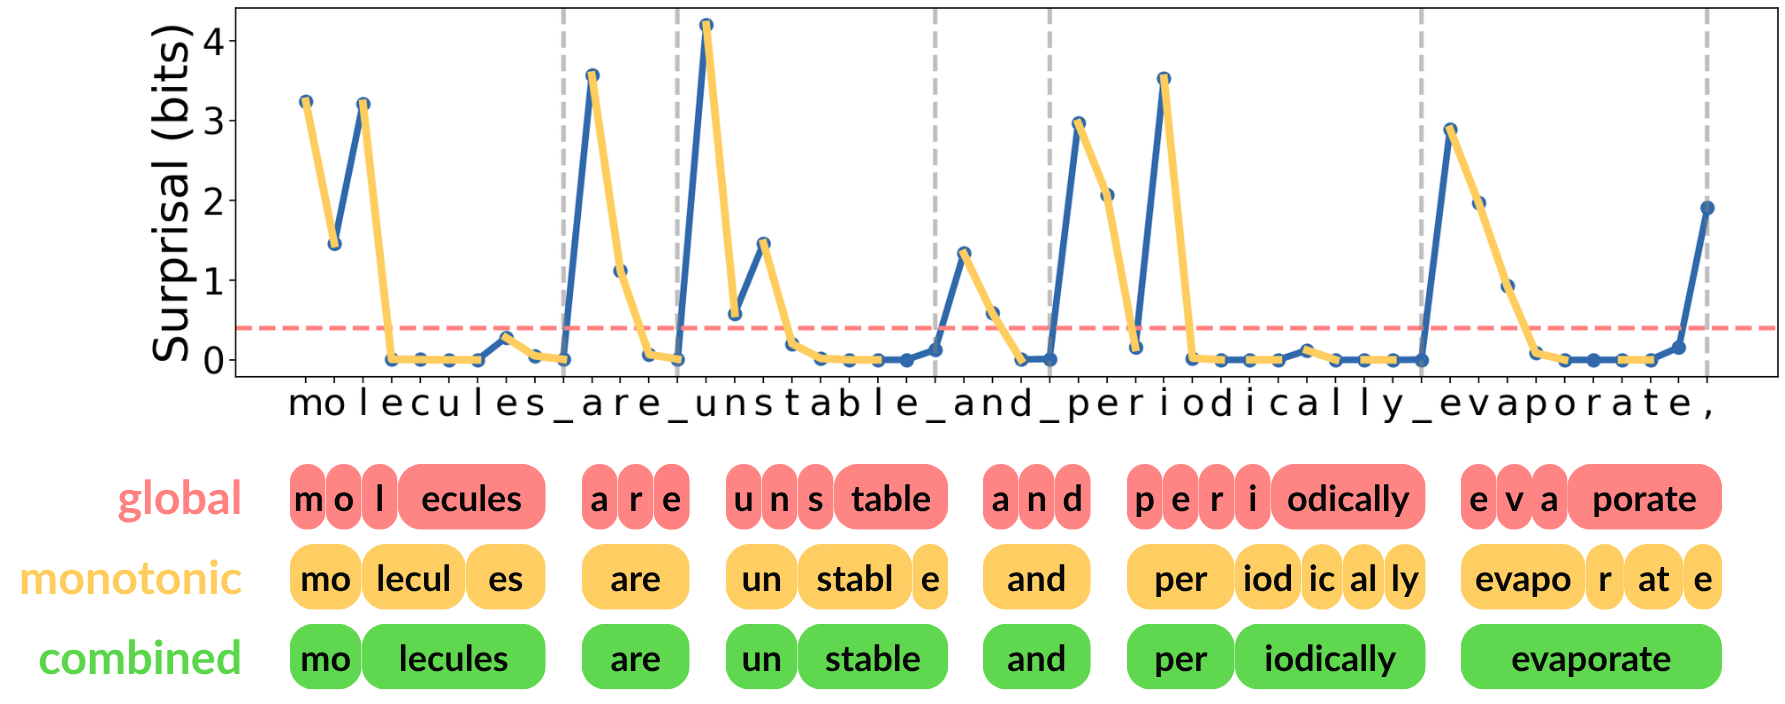
\includegraphics[width=0.7\linewidth]{14Modelling/example.png}
    \caption{An illustration of the three transformations that can be made to convert text input to a phoneme-based input representation.}
    \label{fig:14-example}
\end{figure}

A full systematic comparison of the three input transformations has not yet been conducted, although past work has investigated a subset of these transformations.  \citet{hahn-baroni-2019-tabula} investigate the effect of removing word boundaries and using a word-level or character-level tokenization, evaluating on several psycholinguistic benchmarks. However, they only used graphemic text from Wikipedia and did not ablate the two transformations, only comparing a word-level model (with word boundaries) to a character-level model (without word boundaries). \citet{nguyen-2022-word-boundaries} extend this work, comparing character-level graphemic input (with and without word boundaries) to character-level phonemic input (with and without word boundaries) by training on the Librispeech corpus \citep{panayotov2015librispeech}. They also compare larger units of tokenization (BPE and word-level) for both graphemic and phonemic text, but only with word boundaries included, missing out on several key combinations. These two studies also use an LSTM network, rather than transformer-based architectures.

Most recently (published concurrently with the work presented in this chapter) \citet{bunzeck-etal-2025-small} compare transformer-based BabyLMs trained using graphemes or phonemes and with or without word boundaries. Their setup is similar, but they do not consider the character tokenisation transformation --- all of their models operate either at the character-level or the phoneme-level, for a total of four combinations. Their results are discussed in \cref{sec:14-discussion}.

This chapter provides the first complete comparison of these three input representation transformations by considering all combinations, leading to new input representations that have not been studied before (such as subword tokenization trained without word boundaries). 

%Another simple heuristic for processing text to be more speech-like is to remove word boundaries. At the simplest level of approximation, some past efforts have studied the effects of removing word boundaries from language models \citep{hahn-baroni-2019-tabula, nguyen-2022-word-boundaries}, finding that LSTM-based models see a marked decrease in performance on several psycholingustic benchmarks. 

% However, these architectures were developed for downstream tasks and not for linguistic theories \citep{baroni-2022-proper}. Before using such models, we must establish the extent to which using standard orthographic text gives language models an advantage over input representations that more closely mimic human speech. 

\section{Experimental setup}\label{sec:14-lmsetup}

Exploring the impact of phoneme-based training requires converting orthographic benchmarks and datasets to a phonemic modality, as described in \cref{sec:14-datapreparation}. The experiments in this chapter utilise the \gpt architecture, introduced in \cref{sec:14-phonemearchitecture}. Each of the eight combinations of transformations is implemented as an individual tokeniser, as described in \cref{sec:14-tokenisers}.

\subsection{Data preparation}\label{sec:14-datapreparation}

The training data and evaluation benchmarks used in this chapter to explore the effect of phoneme-based training were first introduced in \cref{sec:12-plausiblepretraining}. Here, the BabyLM dataset is used to compare the effect of the three input representation transformations and \ipachildes, introduced in \cref{chapter:resources}, is used to establish the scaling of phoneme LMs at small data scales. In order to evaluate the models trained on the BabyLM dataset, three benchmarks are used; BLiMP, which tests for linguistic generalisation using minimal pairs, GLUE, which tests for language understanding using fine-tuning tasks, and BabySLM, which uses minimal pairs to test syntactic and lexical generalisation specifically for models trained on developmentally-plausible corpora. BabySLM is also used as the benchmark for the scaling experiments.

The BabyLM dataset, BLiMP and GLUE need to be converted to a phoneme representation in order to be suitable for training and evaluating phoneme-based LMs. This is done using \gpp, as introduced in \cref{chapter:resources}, using the \myemph{phonemizer} backend with the \myemph{en-us} language code, matching the configuration used to generate the EnglishNA section of \ipachildes. Word boundaries are maintained, as these can be removed by the tokenisers implementing the word boundary removal transformation on-the-fly, as explained in \cref{sec:14-tokenisers}. This setup is used to convert each test instance in the evaluation benchmarks to phonemes. Note that the BabySLM benchmark already contains parallel phonemic and orthographic test instances, so does not need to be converted using \gpp.

The same setup is also used to convert the BabyLM dataset. In addition to G2P, minoir cleaning operations are also applied, removing extraneous spaces and formatting anomalies using regular expressions. The parallel dataset containing both the cleaned orthographic text and the generated phonemic format is hosted on Huggingface.\footnote{\href{https://huggingface.co/datasets/phonemetransformers/IPA-BabyLM}{\myemph{huggingface.co/datasets/phonemetransformers/IPA-BabyLM}}}

Crucially, G2P removes punctuation marks, as they are an artefact of orthographic text and equivalent information in speech would be conveyed through prosody, stress, or non-linguistic signals such as gestures, none of which are included in this phonemic format. This has potential consequences for downstream tasks that rely on such markers, as discussed in \cref{sec:14-punctuation}.

\subsection{Phoneme LM architecture}\label{sec:14-phonemearchitecture}

\begin{figure}[t]
    \centering
    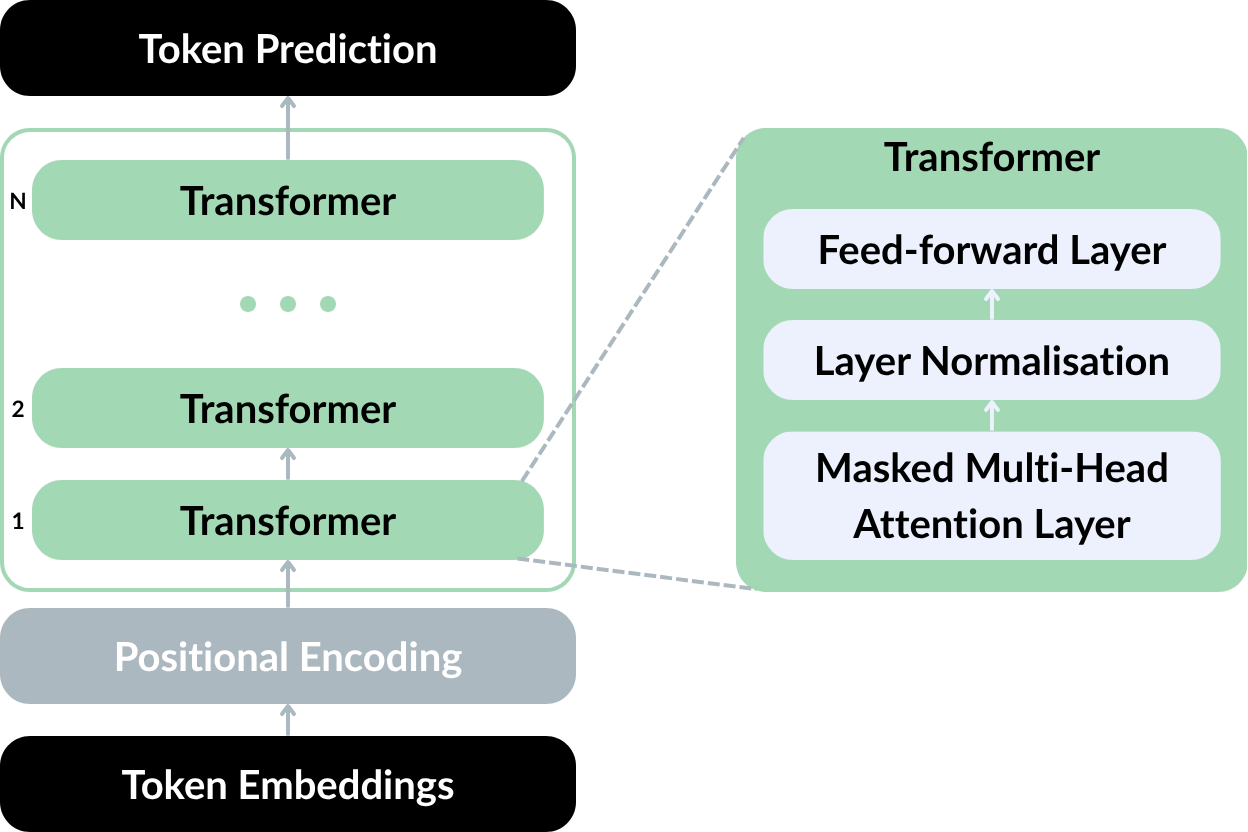
\includegraphics[width=0.7\linewidth]{14Modelling/gpt2.png}
    \caption{An illustration of the \gpt architecture.}
    \label{fig:14-gpt2}
\end{figure}

\gpt is a transformer-based architecture introduced by \citet{radford-2019-gpt2}. It is often called a \emph{decoder-only} architecture, as its transformer blocks resemble the decoder blocks used in the original transformer architecture introduced by \citet{vaswani2017attention}. The model first consists of an embedding layer, after which embeddings are combined with learned position embeddings. These embeddings are then passed through transformer blocks, each of which contains a multi-headed attention layer, a normalisation layer and a feed-forward layer, as illustrated in \cref{fig:14-gpt2}.

\gpt is an auto-regressive model trained with the causal language modelling task --- next-token prediction. The self-attention layer uses a directional mask to ensure that for each position $t$ in a sequence, the token at position $t$ can only attend to positions $\leq t$.  

The output of the final transformer block is passed to a token prediction layer, which for each position, provides a probability distribution over the possible tokens at that position, following the language modelling equation. This can be used for text generation or estimating the probability of input sentences, or this layer can be replaced by a label prediction layer for fine-tuning on downstream tasks.

Here, \gpt models across seven sizes are considered, ranging from 400k parameters to 85M parameters, as summarised in \cref{tab:14-model_sizes}. Following the conventions of the Pythia suite of models \citep{biderman2023pythia}, the number of non-embedding parameters are reported. Unlike their suite, where models are named according to the number of parameters, here models are only referenced according to the number of non-embedding parameters. This is because the same architecture is used with different tokenisers, each of which has a different vocabulary size according to the number of, which alters the number of embedding parameters. The \q{1}{\million}, \q{19}{\million} and \q{85}{\million}-parameter LMs are equivalent to \myemph{Pythia-14M}, \myemph{Pythia-70M} and \myemph{Pythia-160M}, respectively. Whereas the Pythia suite contains much larger models to study the scaling properties at larger scales, here smaller models are implemented in order to study the scaling properties of phoneme LMs trained on smaller phonemic datasets.

% We describe the model and training parameters in \cref{table:baseline_hyperparams}. The model parameters were chosen to match those of the Pythia-170M model from the Pythia suite \citep{biderman2023pythia}. The model has 85M non-embedding parameters and is also equivalent in size to GPT-Neo 125M and OPT-125M. The Pythia models use the GPTNeoX architecture which is slightly different to GPT-2. In initial experiments, we found that GPT-2 performed better on the benchmarks across all eight of our conditions. 


The default training parameters are provided in \cref{tab:14-trainingparams}. During training, data is prepared into batches by first tokenising the entire dataset, combining all tokens into one long vector, then splitting the vector into chunks of \integer{128} tokens. Only the very last example is padded, if required. At each step during training, random chunks are selected and combined into batches. Checkpoints are taken at every \q{10}{\percent} of training, with the best checkpoint chosen at the end of training according to perplexity on a held-out validation set.%Our training scripts are available \href{https://github.com/codebyzeb/PhonemeTransformers}{here}.

% We train the model using all eight tokenizers (using the phonemized dataset for the phoneme-based tokenizers) for 400k steps, selecting the checkpoint with the lowest perplexity.\footnote{The best checkpoint for five of the eight models was the final checkpoint but a visual inspection of the curve revealed that differences between the final checkpoints were minimal.} See \cref{app:14-implementation_details} for a full description of the chosen model parameters and training procedure.

\begin{table}[t]
    \begin{minipage}{.5\linewidth}
        \centering
        \small
        \begin{tabular}{cccccc}
            \toprule
            Model Size & Layers & Heads & Embd & Inner \\
            \midrule
            400k & 2 & 4 & 128 & 512 \\ 
            600k & 3 & 4 & 128 & 512 \\ 
            800k & 4 & 4 & 128 & 512 \\ 
            1M & 6 & 4 & 128 & 512 \\ 
            5M & 6 & 8 & 256 & 1024 \\ 
            19M & 6 & 8 & 512 & 2048 \\ 
            % 25M & 8 & 8 & 512 & 2048 \\ 
            85M & 12 & 12 & 768 & 3072 \\ 
            \bottomrule
        \end{tabular}
        \caption{Parameters for \gpt model of varying sizes. Where values are not reported, they may be assumed to be default values.}
        \label{tab:14-model_sizes}
    \end{minipage}
    \hfill
    \begin{minipage}{.5\linewidth}
        \centering
        \small
        \begin{tabular}{lr}
            \toprule
            Parameter & Value \\
            \midrule
            Max Example Length & 128 \\
            Learning Rate & 0.001\\
            Optimizer & AdamW \\
            Scheduler Type & Linear\\
            Max Steps & 200k \\
            Warm-up Steps & 60k \\
            Per Device Batch Size & 32 \\
            \bottomrule
        \end{tabular}
        \caption{Hyperparameter settings for training the \gpt architecture. Vocabulary size varies according to the tokeniser, but all other parameters are constant across experiments. Where values are not reported, they may be assumed to be default values.}
        \label{tab:14-trainingparams}
    \end{minipage}
\end{table}

\subsection{Tokenisers}\label{sec:14-tokenisers}

The eight combinations of input transformations are implemented as individual tokenisers using \myemph{Huggingface Tokenizers}. Each tokeniser either applies (\cmark) or does not apply (\xmark) each transformation as follows:

\begin{itemize}
\setlength\itemsep{0.1em}
    \item \characterhighlight{Character tokenization} A character-based tokeniser is constructed using a vocabulary extracted from the data (\cmark) or a subword-based tokeniser is implemented using BPE (\xmark).
    \item \spacehighlight{Word boundary removal} The tokeniser's normaliser strips whitespace (\cmark) or no normaliser is applied to maintain whitespace (\xmark).
    \item \phonemehighlight{Phonemic transcription} The tokenizer is either trained on a phonemic version of the dataset (\cmark) or on the original orthographic version (\xmark).
\end{itemize}

Note that for the combination of BPE and no word boundaries, the whitespace is removed before training, so the model may learn `subwords' that cross word boundaries.

Each tokeniser also adds a dedicated ``utterance boundary'' token \texttt{UTT\_BOUNDARY} to the start of each sentence, representing the pauses between spoken utterances and serving as a dedicated start-of-sentence token. When sentences are collated, it also implicitly acts as an end-of-sentence token, as discussed in \cref{sec:14-endofsentence}.

For each of the eight combinations of the three transformations, a tokenizer is trained on the `train' portion of the BabyLM dataset. For the subword-based models, a vocabulary size of 16k is used to train BPE --- matching the vocabulary size used by the two BabyLM challenge baseline models (described below). The output of all eight tokenisers is illustrated in \cref{table:results}. The tokeniser implementing none of the transformations is the standard subword-based input representation typically used to train language models, whereas the tokeniser with all three transformations applied is the phoneme-based input representation.

Note that the vocabulary size for the character-level tokenizers operating on phonemes is less than half the vocabulary size of their orthographic equivalents. This is because the phonemic data only consists of the 47 phonemes produced by the North American English accent, but orthographic characters also include numbers, punctuation and other symbols. 

\begin{table*}[t]
    \centering
    \footnotesize
    \addtolength{\tabcolsep}{-0.2em}
    \begin{tabular}{l||ccc|c|c||ccccc}
       Model & \rotatebox[origin=l]{90}{\characterhighlight{Character tokenization}} & \rotatebox[origin=l]{90}{\spacehighlight{Word boundary removal}} & \rotatebox[origin=l]{90}{\phonemehighlight{Phonemic transcription}} & \rotatebox[origin=l]{90}{Vocabulary Size} & Example Tokenization & \rotatebox[origin=l]{90}{BLiMP Filtered} & \rotatebox[origin=l]{90}{BLiMP Supplement} & \rotatebox[origin=l]{90}{GLUE} & \rotatebox[origin=l]{90}{BabySLM (Syntactic)} & \rotatebox[origin=l]{90}{BabySLM ( Lexical)} \\
       \midrule
        Baby Llama & \xmark & \xmark & \xmark & \q{16}{\thousand} & ~\mybox{\textvisiblespace what} ~\mybox{\textvisiblespace a} ~\mybox{\textvisiblespace con} ~\mybox{und} ~\mybox{rum} ~\mybox{\textvisiblespace !} & 73.1 & 60.6 & 69.0 &  94.0 & - \\
        LTG-BERT & \xmark & \xmark & \xmark & \q{16}{\thousand} & ~\mybox{\textvisiblespace what} ~\mybox{\textvisiblespace a} ~\mybox{\textvisiblespace con} ~\mybox{und} ~\mybox{r} ~\mybox{um} ~\mybox{\textvisiblespace !} & 69.3 & 66.5 & 68.4 & 75.8 & - \\
        \midrule
         & \xmark & \xmark & \xmark & \q{16}{\thousand} & ~\mybox{\textvisiblespace what} ~\mybox{\textvisiblespace a} ~\mybox{\textvisiblespace con} ~\mybox{und}  ~\mybox{rum} ~\mybox{\textvisiblespace!} & \textbf{77.8} & \textbf{69.4} & \textbf{71.6} & 92.8 & - \\
         & \xmark & \spacehighlight{\cmark} & \xmark & \q{16}{\thousand} & \mybox{what} ~\mybox{acon} ~\mybox{un} ~\mybox{drum} ~\mybox{!} & 73.9 & 64.3 & 68.6 & 73.9 & - \\
         & \xmark & \xmark & \phonemehighlight{\cmark} & \q{16}{\thousand} & ~\mybox{\textvisiblespace \textipa{w2t}} ~\mybox{\textvisiblespace \textipa{2}} ~\mybox{\textvisiblespace \textipa{k@n}} ~\mybox{\textipa{2nd}} ~\mybox{\textipa{\*r@m}} & 74.7 & 59.6 & 68.6 & 85.8 & 67.3 \\
         \multirow{2}{*}{\gpt} & \xmark & \spacehighlight{\cmark} & \phonemehighlight{\cmark} & \q{16}{\thousand} & ~\mybox{\textipa{w2t}} ~\mybox{\textipa{2k@n}} ~\mybox{\textipa{2nd}} ~\mybox{\textipa{\*r@m}} & 71.7 & 56.7 & 65.5 & 74.7 & 71.2  \\
         & \characterhighlight{\cmark} & \xmark & \xmark & \integer{115} & \makecell{ \mybox{w} ~\mybox{h} ~\mybox{a} ~\mybox{t} ~\mybox{\textvisiblespace } ~\mybox{a} ~\mybox{\textvisiblespace } \\ ~\mybox{c} ~\mybox{o} ~\mybox{n} ~\mybox{u} ~\mybox{n} ~\mybox{d} ~\mybox{r} ~\mybox{u} ~\mybox{m} ~\mybox{\textvisiblespace } ~\mybox{!}} & 77.4 & 63.6 & 64.4 & \textbf{94.9} & - \\
         & \characterhighlight{\cmark} & \spacehighlight{\cmark} & \xmark & \integer{114} & \makecell{\mybox{w} ~\mybox{h} ~\mybox{a} ~\mybox{t} ~\mybox{a} \\ ~\mybox{c} ~\mybox{o} ~\mybox{n} ~\mybox{u} ~\mybox{n} ~\mybox{d} ~\mybox{r} ~\mybox{u} ~\mybox{m} ~\mybox{!}} & 75.1 & 64.8 & 64.8 & 88.3 & - \\
         & \characterhighlight{\cmark} & \xmark & \phonemehighlight{\cmark} & \integer{51} & \makecell{\mybox{w} ~\mybox{\textipa{2}} ~\mybox{\textipa{t}} ~\mybox{\textvisiblespace } ~\mybox{\textipa{2}}  ~\mybox{\textvisiblespace } \\ ~\mybox{\textipa{k}} ~\mybox{\textipa{@}} ~\mybox{\textipa{n}} ~\mybox{\textipa{2}} ~\mybox{n} ~\mybox{d} ~\mybox{\textipa{\*r}} ~\mybox{\textipa{@}} ~\mybox{m}} & 74.7 & 58.5 & 65.6 & 90.5 & \textbf{89.6}  \\
         & \characterhighlight{\cmark} & \spacehighlight{\cmark} & \phonemehighlight{\cmark} & \integer{50} & \makecell{\mybox{w} ~\mybox{\textipa{2}} ~\mybox{\textipa{t}} ~\mybox{\textipa{2}} \\ ~\mybox{\textipa{k}} ~\mybox{\textipa{@}} ~\mybox{\textipa{n}} ~\mybox{\textipa{2}} ~\mybox{n} ~\mybox{d} ~\mybox{\textipa{\*r}} ~\mybox{\textipa{@}} ~\mybox{m}} & 72.5 & 57.6 & 65.4 & 83.9 & 87.8
    \end{tabular}
    \caption{Results for the two BabyLM baseline models and the \gpt model trained under all eight conditions. On the left, the effects of each of the three transformations across all eight possible combinations are visualised by tokenising the example phrase ``what a conundrum!''. The `\textvisiblespace ' character denotes word boundaries. On the right, the BLiMP, GLUE and BabySLM scores achieved by each model are reported, with the best scores in each column in \textbf{bold}.} %Note that the BabySLM Lexical score can only be computed for models trained with phonemic input.}
    \label{table:results}
\end{table*}

\section{Experiment: Phoneme-based pre-training}\label{sec:14-phonemepretraining}

This experiment explores the impact of phoneme-based pre-training by training a set of models that only differ according to the input representation. The \q{85}{\million}-parameter \gpt model is trained using each of the eight tokenisers (using the phonemic data for the phoneme-based tokenisers), using the training procedure described in \cref{sec:14-phonemearchitecture}.\footnote{As these models are larger and trained on more data, \q{400}{\thousand} steps are used, with a warmup of \q{90}{\thousand}.} The only difference during training is the tokeniser used, allowing the effect of the input representation to be established through evaluation on BLiMP, GLUE and BabySLM. The trained models are hosted on Huggingface, along with the eight tokenisers.\footnote{\href{https://huggingface.co/collections/phonemetransformers/from-babble-to-words-66e068b54765a48ff30273c9}{\myemph{huggingface.co/collections/phonemetransformers/from-babble-to-words-66e068b54765a48ff30273c9}}}

Two baseline models are used; the best-performing models from the first edition of the BabyLM challenge. These are \myemph{Baby Llama}, an auto-regressive model trained using knowledge distillation from an ensemble of teachers \citep{timiryasov-tastet-2023-baby}, and \myemph{LTG-BERT}, an architectural variation of the standard auto-encoding \bert architecture optimized for small, speech-based corpora \citep{samuel-etal-2023-trained, charpentier-samuel-2023-layers}. Both models use a \bpe tokenizer with a vocabulary size of \q{16}{\thousand} and were trained on the BabyLM dataset by the organisers of the BabyLM challenge, acting as official baselines for the second edition of the challenge \citep{hu-etal-2024-findings}. Both models are similar in size to the \gpt model used here --- \myemph{Baby Llama} has \q{41}{\million} non-embedding parameters and \myemph{LTG-BERT} has \q{110}{\million}.

\subsection{Results}

\Cref{table:results} summarises the results obtained by the two baseline models and the \gpt model trained in all eight conditions. %Due to limited computational resources, only a single run per condition is trained for each condition, limiting significance testing. However, general trends can still be observed. 
The base \gpt model with no input adjustments outperforms the two baselines for BLiMP, BLiMP Supplement and GLUE, validating the choice of training hyper-parameters and \gpt as a model architecture.

Comparing the \gpt model with no input transformations (top row) to the same model with all three transformations applied (bottom row), we notice a decrease in performance across all benchmarks. Although this indicates that the \gpt architecture is best suited for the standard orthographic input representation (word boundaries, graphemes and subword tokenisation), the decrease in performance when the three transformations are applied is not substantial and scores remaining competitive with the baseline models (all combinations still outperform \myemph{LTG-BERT} on BLiMP). It is clear that the \gpt architecture is still capable of learning grammatical rules and excelling at downstream tasks when the input consists of individual phonemes with no word boundaries, indicating that transformer-based architectures are robust to alternative input representations.

\Cref{sec:14-effect} investigates this result further through an ablation of the three transformations, noting the effect of punctuation and context size. \Cref{sec:14-babyslm} focuses on the BabySLM metrics, which demonstrate a different pattern to the other benchmarks. Finally, \cref{sec:14-punctuation} investigates the consequences of removing punctuation.

\subsection{Teasing apart the three transformations}\label{sec:14-effect}

Since the \gpt model was trained with all eight combinations of the three input adjustments, the effect of each transformation can be teased apart.

\begin{figure}
    \centering
    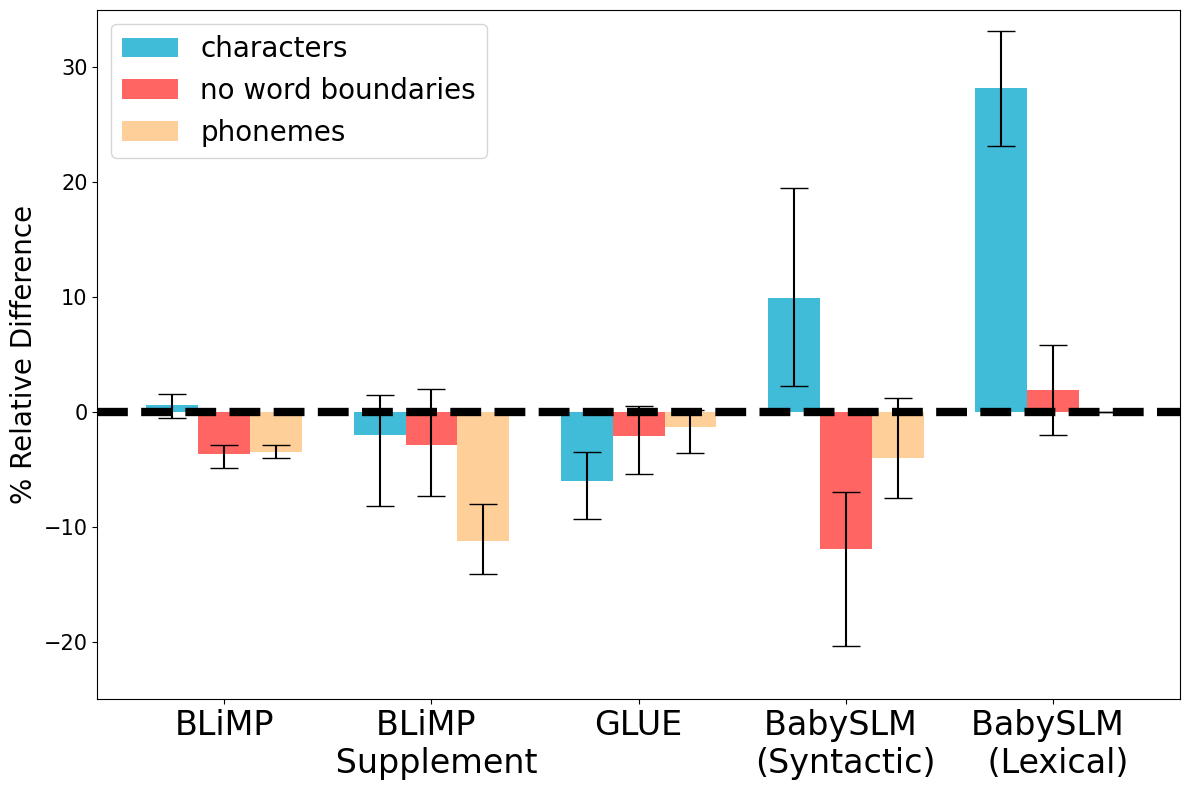
\includegraphics[width=0.7\linewidth]{14Modelling/confidence-int.png}
      \caption{Mean (with Min and Max range) percentage difference achieved on each benchmark's macro score as a result of the three adjustments.}
    \label{fig:14-condition-differences}
\end{figure}

\begin{table}[t]
    \centering
    \small
    \begin{tabular}{lcccc}
        \toprule
        & BLiMP& \makecell{BLiMP \\ Supplement} & GLUE & \makecell{BabySLM \\ (Syntactic)} \\
        \midrule
        \makecell{orthographic vs. phonemic} & \textbf{0.0001} & 0.0780 & \textbf{0.0149} & 0.1884 \\
        \makecell{word boundaries vs. no word boundaries} & \textbf{0.0000} & 0.1831 & 0.0813 & \textbf{0.0118} \\
        \makecell{character vs. subword} & 0.5069 & 0.4832 & \textbf{0.0010} & 0.1500 \\
        \bottomrule
    \end{tabular}
    \caption{$p$-values from the paired student t-tests for each experiment. Significant results are given in \textbf{bold} using an alpha level of 0.05.}
    \label{tab:14-pvalues}
\end{table}

Each transformation can group four pairs of runs that only differ with respect to that transformation (e.g. the four runs with a phonemic transcription and the four runs with orthographic text). For each pair, the percentage increase in each metric caused by the transformation is calculated. The average of these four percentage differences are shown in \cref{fig:14-condition-differences}.

It is difficult to determine whether the results for a given benchmark are significant given that only a single model is trained for each of the eight conditions (due to computational constraints). Instead, significance can be computed by comparing the  scores for each subtask within a benchmark. For each transformation, paired results for each subtask can be created by averaging the scores achieved by the four models with and without the transformation applied. A paired student $t$-test can then assess the significance of the transformation. The $p$-values for these significance tests are provided \cref{tab:14-pvalues}. Note that there are 67 subtasks for BLiMP, 5 for BLiMP Supplement, 9 for GLUE and 9 for BabySLM (Syntactic). With only 5 pairs for BLiMP Supplement, the test is under-powered and low $p$-values are unlikely. There are no subtasks for BabySLM (Lexical) so significance cannot be computed in the same way. 

These results are used to identify the effect of each transformation, as discussed below.

\paragraph{Character tokenisation} Character tokenisation leads to decreased exposure during training since each sentence is represented with more tokens, increasing the number of steps required for each epoch. Despite this, character tokenisation does not significantly decrease performance on BLiMP or BLiMP Supplement compared to subword tokenization. This validates previous work which found that despite the higher computation costs, character-based language models are just as capable of learning language \citep{al-rfou_character-level_2019, hahn-baroni-2019-tabula}. There is a significant decrease for GLUE but this is likely due to the fact that many of the fine-tuning examples for GLUE are very long and the model's context size is only 128 tokens, leading to severe truncation. As character-based tokenisers output more tokens for the same sentence than \bpe subword tokenisers, this means that for many GLUE tasks, necessary information is lost.

\paragraph{Word boundary removal} Removing word boundaries significantly decreases the BLiMP score, but the decreases for BLiMP Supplement and GLUE are not significant. In their investigation, \citet{nguyen-2022-word-boundaries} found a decrease of 7-8\% on their own phonemic version of BLiMP when word boundaries were removed, but here there is only an average decrease of 3.7\%. As they only trained 3-layer LSTMs, it is possible that larger models like \gpt are more robust to the loss of word boundaries.

\paragraph{Phonemic transcription} Finally, using a phonemic transcription instead of the original written text significantly decreases performance on BLiMP and GLUE, although the percentage decreases are small (3.5\% and 1.5\% respectively). It also leads to the largest decrease of 11.3\% for BLiMP Supplement. A possible explanation for this particular decrease in explored in \cref{sec:14-punctuation}.

\subsection{BabySLM}
\label{sec:14-babyslm}

In their study, \citet{lavechin} achieved their highest syntactic score of \integer{70.4} using \babyberta \citep{huebner-etal-2021-babyberta} trained on only \q{5}{\million} words from CHILDES \citep{macwhinney1985child}. All eight \gpt models trained here beat this score, with the best score of \integer{94.9} achieved by the model that uses character-based tokenization (on written text, with word boundaries). This is contrast to the other benchmarks, where the standard subword-based representation leads to the highest score (note that \babyberta also uses a subword-based input representation). There is also an architectural difference: \babyberta is an auto-encoder trained using MLM, whereas \gpt model is auto-regressive, using next-token prediction. The \myemph{LTG-BERT} baseline, which is a similarly sized model also trained on \q{100}{\million} words, only achieves a score of \integer{75.8}. The \myemph{Baby Llama} baseline, by comparison, achieves \integer{94.0}. It is possible that the auto-regressive architecture is much more suited to the syntactic task than the auto-encoder architecture of \bert. 

When it comes to the lexical test, the highest score achieved by \citet{lavechin} was \integer{75.4} using a 3-layer LSTM trained on \q{1.2}{\million} words from the Providence corpus \citep{borschinger-etal-2013-joint} which they converted to phonemes using \myemph{phonemizer}. Here, the highest scoring model was also trained with character-based tokenisation of phonemes, but did include word boundaries, achieving a score of \integer{89.6}. The model without word boundaries got the second-highest score with \integer{87.8}.

Note that \gpt is larger (12 layers) and trained on much more data \q{100}{\million} words than the two BabySLM baselines. The BabyLM dataset also contains a wider variety of sentences than just the child-directed utterances in CHILDES. The effect of model size and data size on BabySLM scores is explored in \cref{sec:14-sizerequirements}, providing a fairer comparison with the results of \citet{lavechin}.

% We are currently investigating the effect of model size and training size on the BabySLM scores. In initial experiments, we found that even a 6-layer model trained on only 7 million words from CHILDES was able to achieve a lexical score of 82, but this model also only achieved a syntactic score of 70. We hypothesize that lexical-level knowledge can be learned with less data and by smaller models when compared to learning syntactic knowledge, but this research is ongoing.

The effect of each transformation is shown in \cref{fig:14-condition-differences}. The phonemic modality on average reduces the syntactic score by 4.0\%, which is in line with the other benchmarks discussed above. Unlike the other benchmarks, the character tokenisation condition always leads to an improvement for both BabySLM scores: an average increase of 9.9\% for the syntactic score and 23.9\% for the lexical score. The sentences used for the syntactic test are all very short compared to the BLiMP sentences (4 words long on average) so a more fine-grained representation may be more effective. For the lexical test, where single words are compared that often only differ by a single phoneme, it seems more appropriate to use a character-based tokenisation as the model needs to learn the distributional properties of individual phonemes, which may be lost in subword units. 

The removal of word boundaries has a contrasting effect on the two scores. It reduces the syntactic score by 11.9\% but increases the lexical score by 1.9\%, the only benchmark where removing word boundaries is a positive change. However, the best individual lexical score was achieved by the model that did include word boundaries, suggesting that word boundaries are a helpful signal for a model learning to distinguish words from non-words, possibly because they help separate short sequences of phonemes that appear across word boundaries but not within words. 

%It is also notable that the decrease in the syntactic score removing word boundaries has a much larger effect for the BPE models (a decrease of 18.9 and 11.1 points) than the character-based models (which both decrease by 6.6). 

\Zeb{Maybe move this below to discussion, since it ties into next chapter. And above as well.}

For the syntactic score, the worst scores are achieved by the models that learn subwords without word boundaries. For these models, \bpe is essentially acting as an unsupervised word segmentation algorithm --- learning to split entire sentences into useful units. Examining the outputs in \cref{table:results}, it seems that with a vocabulary size of \q{16}{\thousand}, \bpe learns learns morpheme-like units such as \ex{un} but also units that cross word boundaries, such as \ex{acon}. The resulting implicit subword boundaries seem to have particular consequences when evaluating the shorter BabySLM sentences. Using the BPE algorithm in this way could be of interest for word segmentation studies. 

\subsection{The effect of punctuation}
\label{sec:14-punctuation}

Punctuation is primarily a feature of orthographic text and so is rarely included in phonemic transcripts. However, punctuation in written text does carry important meaning about the structure and tone of sentences, which in speech, would typically be conveyed through intonation, stress and rhythm. Although words are maintained across both modalities, stripping punctuation may be removing valuable information that is used by LMs to learn and process language. 

In some instances, na\"ively stripping punctuation can even lead to nonsense sentences. This may explain the large dip in performance for BLiMP Supplement, as three of the five subtasks rely on punctuation to simulate question-answer pairs or dialogue, such as:

\begin{center}
\texttt{A: What did you break?\textbackslash nB: I broke a bowl.}
\end{center}

In the example above, the line break, colon and question mark are used to indicate speaker turns and convey the question-answer nature of the prompt. Removing the punctuation leads to a nonsense sentence, especially when read aloud with no pauses or change in tone to indicate the structure:

\vspace{-1mm}
\begin{center}
\textipa{2}~\textvisiblespace~\textipa{w 2 t}~\textvisiblespace~\textipa{d I d}~\textvisiblespace~\textipa{j u:}~\textvisiblespace~\textipa{b}~\textipa{\*r}~\textipa{eI k}~\textvisiblespace~\textipa{b i:}~\textvisiblespace~\textipa{aI}~\textvisiblespace\\~\textipa{b~\*r~o~U~k}~\textvisiblespace~\textipa{2}~\textvisiblespace~\textipa{b oU l}~\textvisiblespace
\end{center}
\vspace{-1mm}

Without punctuation, the names \ex{A} and \ex{B} seem out of place. A model trained on written text can use punctuation to possibly understand that these are names, but a spoken model without punctuation would struggle to process this sentence. This reliance on punctuation seems to be the leading cause of the drop in performance on BLiMP Supplement seen in \cref{fig:14-condition-differences}. By removing the three subtasks where punctuation plays a key role in structuring the sentence pairs, the decrease in performance caused by the phonemic transformation reduces from \q{11.3}{\percent} to \q{0.9}{\percent}.

There is another subtle yet crucial consequence of removing punctuation: stripping punctuation at the end of sentences, if not handled correctly, can lead to significant decreases in performance on these benchmarks. This is discussed in the next section.

\subsection{The effect of end-of-sentence tokens}\label{sec:14-endofsentence}

By default, our tokenizers add a special start-of-sentence token \texttt{UTT\_BOUNDARY} to all sentences. This corresponds to the \texttt{<s>} token often used by tokenizers to help LMs with sentence-level processing, and also represents utterance boundaries, which unlike word boundaries are a clear cue present in speech and often included in word segmentation studies \citep{feliciano-de-faria-2019-utterance-boundaries}. 

Since sentences are collated together during training, this means that these tokens also appear at the end of every sentence, implicitly acting as end-of-sentence tokens. As a result, the model may use them to represent sentence-level information (especially given that these models are auto-regressive). However, in most evaluation tasks, sentences are presented individually (with padding) and so by default the tokeniser does not add this token to the end of sentences. 

\begin{table*}[t]
    \centering
    \small
    \begin{tabular}{ccc}
        \toprule
        & Grammatical & Ungrammatical \\
        \midrule
       Original & \makecell{Patrick revealed what \\ a lot of men wore.} & \makecell{Patrick revealed that \\ a lot of men wore.} \\
       \midrule
       \makecell{\bpe \\ (Orthographic)} & \makecell{\mybox{<s>}~~\mybox{\textvisiblespace patrick}~~\mybox{\textvisiblespace revealed}~ \mybox{\textvisiblespace what}\vspace{2pt}\\ ~\mybox{\textvisiblespace a}~~\mybox{\textvisiblespace lot}~~\mybox{\textvisiblespace of}~~\mybox{\textvisiblespace men}~~\mybox{\textvisiblespace wore}~~\mybox{\textvisiblespace .}} & \makecell{\mybox{<s>}~~\mybox{\textvisiblespace patrick}~ \mybox{\textvisiblespace revealed}~ \mybox{\textvisiblespace that}\vspace{2pt}\\ ~\mybox{\textvisiblespace a}~~\mybox{\textvisiblespace lot}~~\mybox{\textvisiblespace of}~~\mybox{\textvisiblespace men}~~\mybox{\textvisiblespace wore}~~\mybox{\textvisiblespace .}} \\
       \midrule
       \makecell{\bpe \\ (Phonemic)} & \makecell{ \mybox{<s>}~~\mybox{\textvisiblespace \textipa{p\ae t\*rIk}}~~\mybox{\textvisiblespace \textipa{\*rIvi:ld}}~~\mybox{\textvisiblespace \textipa{w2t}}\vspace{2pt}\\~~\mybox{\textvisiblespace \textipa{2}}~~\mybox{\textvisiblespace\textipa{lAt}} ~~\mybox{\textvisiblespace \textipa{2v}}~~\mybox{\textvisiblespace \textipa{mEn}}~~\mybox{\textvisiblespace \textipa{wO\*r}}} & \makecell{ \mybox{<s>}~~\mybox{\textvisiblespace \textipa{p\ae t\*rIk}}~~\mybox{\textvisiblespace \textipa{\*rIvi:ld}}~~\mybox{\textvisiblespace \textipa{T\ae t}}\vspace{2pt}\\~~\mybox{\textvisiblespace \textipa{2}}~~\mybox{\textvisiblespace\textipa{lAt}} ~~\mybox{\textvisiblespace \textipa{2v}}~~\mybox{\textvisiblespace \textipa{mEn}}~~\mybox{\textvisiblespace \textipa{wO\*r}}} \\
       \bottomrule
    \end{tabular}
    \caption{An example sentence pair from the \texttt{wh\_vs\_that\_with\_gap} subtask in BLiMP and the outputted tokens from our two tokenizers that use subwords but do not remove word boundaries. The `\textvisiblespace ' character denotes word boundaries and the `<s>' token represents the \texttt{UTT\_BOUNDARY} token which acts as an utterance boundary and a start-of-sentence token.}
    \label{tab:14-blimpexample}
\end{table*}

This has consequences for zero-shot evaluation tasks where the grammaticality of the sentence depends on the sentence being marked as complete, which is the case for several of the BLiMP subtasks. For instance, one subtask evaluates a model's understanding of filler-gap dependencies by presenting grammatical \ex{wh}-phrases with \ex{that}-phrases that are ungrammatical due to a missing dependency. An example is given in \cref{tab:14-blimpexample} along with the tokens produced by two of our tokenizers. Crucially, the phonemic transcriptions do not include punctuation (see \cref{sec:14-punctuation}) and for this task, without an end-of-sentence marker, the ``ungrammatical'' sentence is no longer ungrammatical, as it could just be incomplete.

This means that the subtask remained a valid test for our orthographic models (due to the inclusion of punctuation to mark the end of the sentence), but not the phonemic ones, since for the phonemic models both the ``grammatical'' and ``ungrammatical'' sentences could be considered grammatical. Since this task is not balanced, any preference for the word ``that'' over the ``wh''-words would lead to the model consistently choosing the ``that'' sentences and achieving results below chance (which is \integer{50} for all BLiMP tasks).

% There is another subtle yet crucial consequence of removing punctuation: stripping punctuation at the end of sentences, if not handled correctly, can lead to significant decreases in performance on these benchmarks. This is because without an end-of-sentence marker, certain evaluation examples are no longer valid. In order to mark the end of the sentences without punctuation, it is important to ensure that the dedicated sentence-separation token is added to the end of each evaluation instance. The effect of this adjustment is highlighted in \cref{fig:14-endofsentencetoken}. The increase in BLiMP score for the phoneme-based LMs confirms that this change is necessary and highlights the importance of carefully investigating the role of tokenisation in the evaluation of LMs. This is discussed further in the next section.

In initial experiments, the phoneme-based LMs achieved scores between \integer{0.06} and \integer{0.14} for this task whereas the orthographic LMs achieved scores between \integer{0.35} and \integer{0.53}. Adding the \texttt{UTT\_BOUNDARY} token to the end of every evaluation resulted in the phoneme-based LMs achieving scores between \integer{0.26} and \integer{0.34} (with little change for the orthographic models). These results also held for several other BLiMP tasks with similar constructions. 

Thus, the end-of-sentence token was added to the end of every evaluation instance for all benchmarks reported in this chapter for two reasons. First, it acts as a necessary end-of-sentence marker to ensure certain tests remain valid for the phonemic models, and second, because the token may encode useful sentence-level information for all models (particularly for GLUE tasks, as only the encoding of the final token is used for predictions).

\begin{figure}[t]
    \centering
    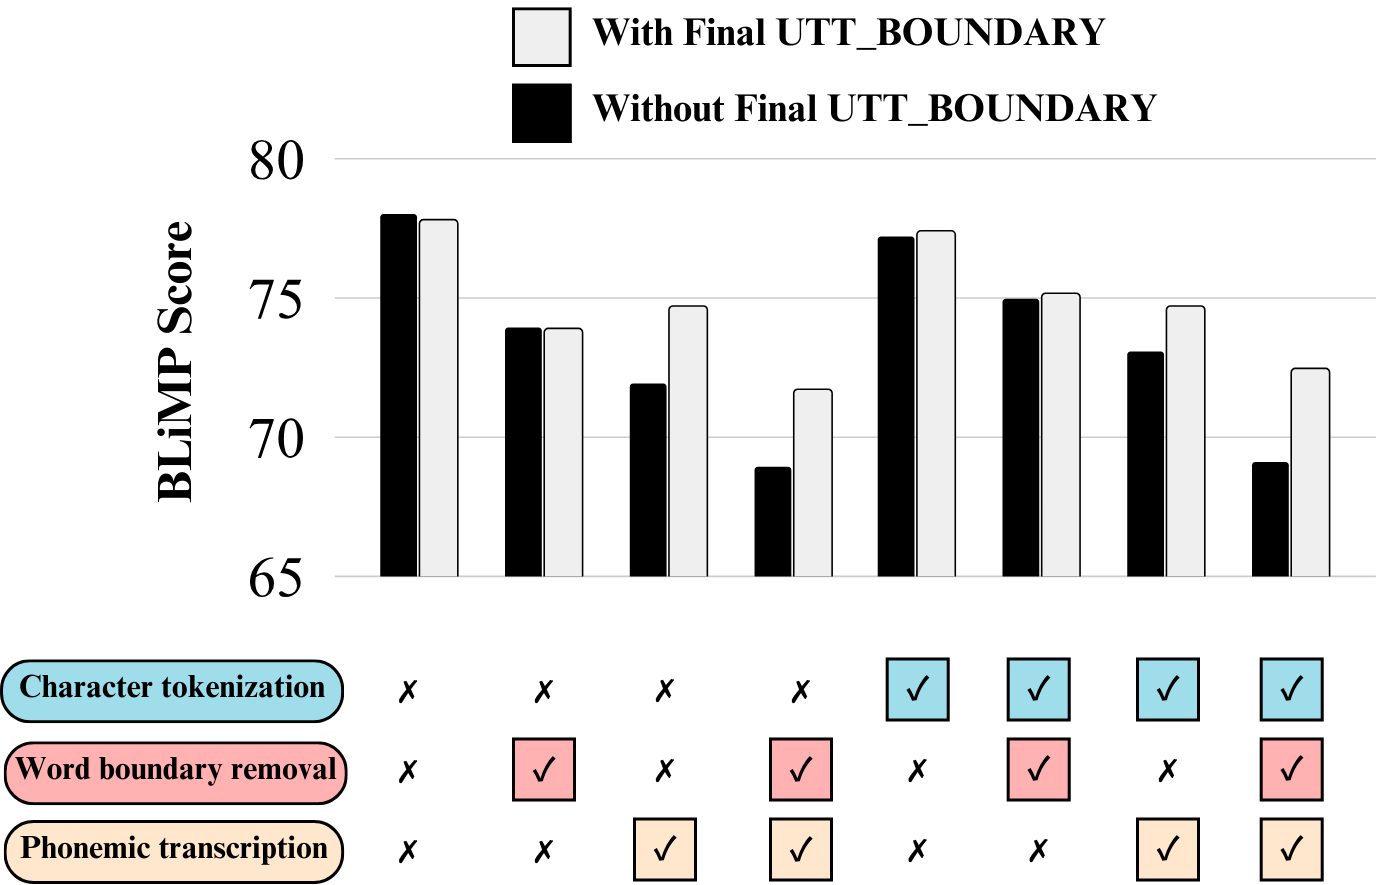
\includegraphics[width=0.7\linewidth]{14Modelling/endofsentencetoken.png}
    \caption{The overall BLiMP scores achieved by \gpt in the eight conditions with and without the \texttt{UTT\_BOUNDARY} token (used to separate sentences) included at the end of evaluation instances.}
    \label{fig:14-endofsentencetoken}
\end{figure}

The effect of this decision is shown in \cref{fig:14-endofsentencetoken} which reports the overall BLiMP scores for the eight conditions with and without the inclusion of the \texttt{UTT\_BOUNDARY} token at the end of each evaluation instance. There is a very large increase for all four phoneme-based LMs with little change for the orthographic LMs, confirming that this was a crucial adjustment and highlighting the importance of carefully investigating the role of tokenisation in the evaluation of LMs.

\section{Experiment: Size requirements of phoneme LMs}\label{sec:14-sizerequirements}

The previous experiment established although LMs trained with a phoneme-based input representation often score lower on benchmarks than when the standard subword-based input representation is used, these phoneme LMs are still capable of learning linguistic generalisations and succeeding at downstream tasks, indicating that phoneme LMs are a useful tool for phonological experimentation. In order to support such experiments, it is important to establish the size requirements of phoneme LMs trained at much smaller scales of data, such as what is available for each language in \ipachildes.

To simulate the smallest and largest languages in \ipachildes while keeping the language consistent, six subsamples of the EnglishNA portion are used, ranging from \q{80}{\thousand} to \q{5}{\million} words. Child-produced utterances and word boundaries are removed, following prior phonological experiments (see \cref{sec:12-phonemic}). A suite of \gpt models is trained on each of these subsets, with the number of non-embedding parameters ranging from \q{80}{\thousand} to \q{5}{\million}, as presented in \cref{sec:14-phonemearchitecture}. To prevent over-fitting, for each combination of model size and data size, three models are trained with dropouts of \integer{0.1}, \integer{0.3} and \integer{0.5}, selecting the model with the lowest perplexity for each.



\begin{figure}[t]
    \centering
    \begin{subfigure}{0.45\linewidth}
        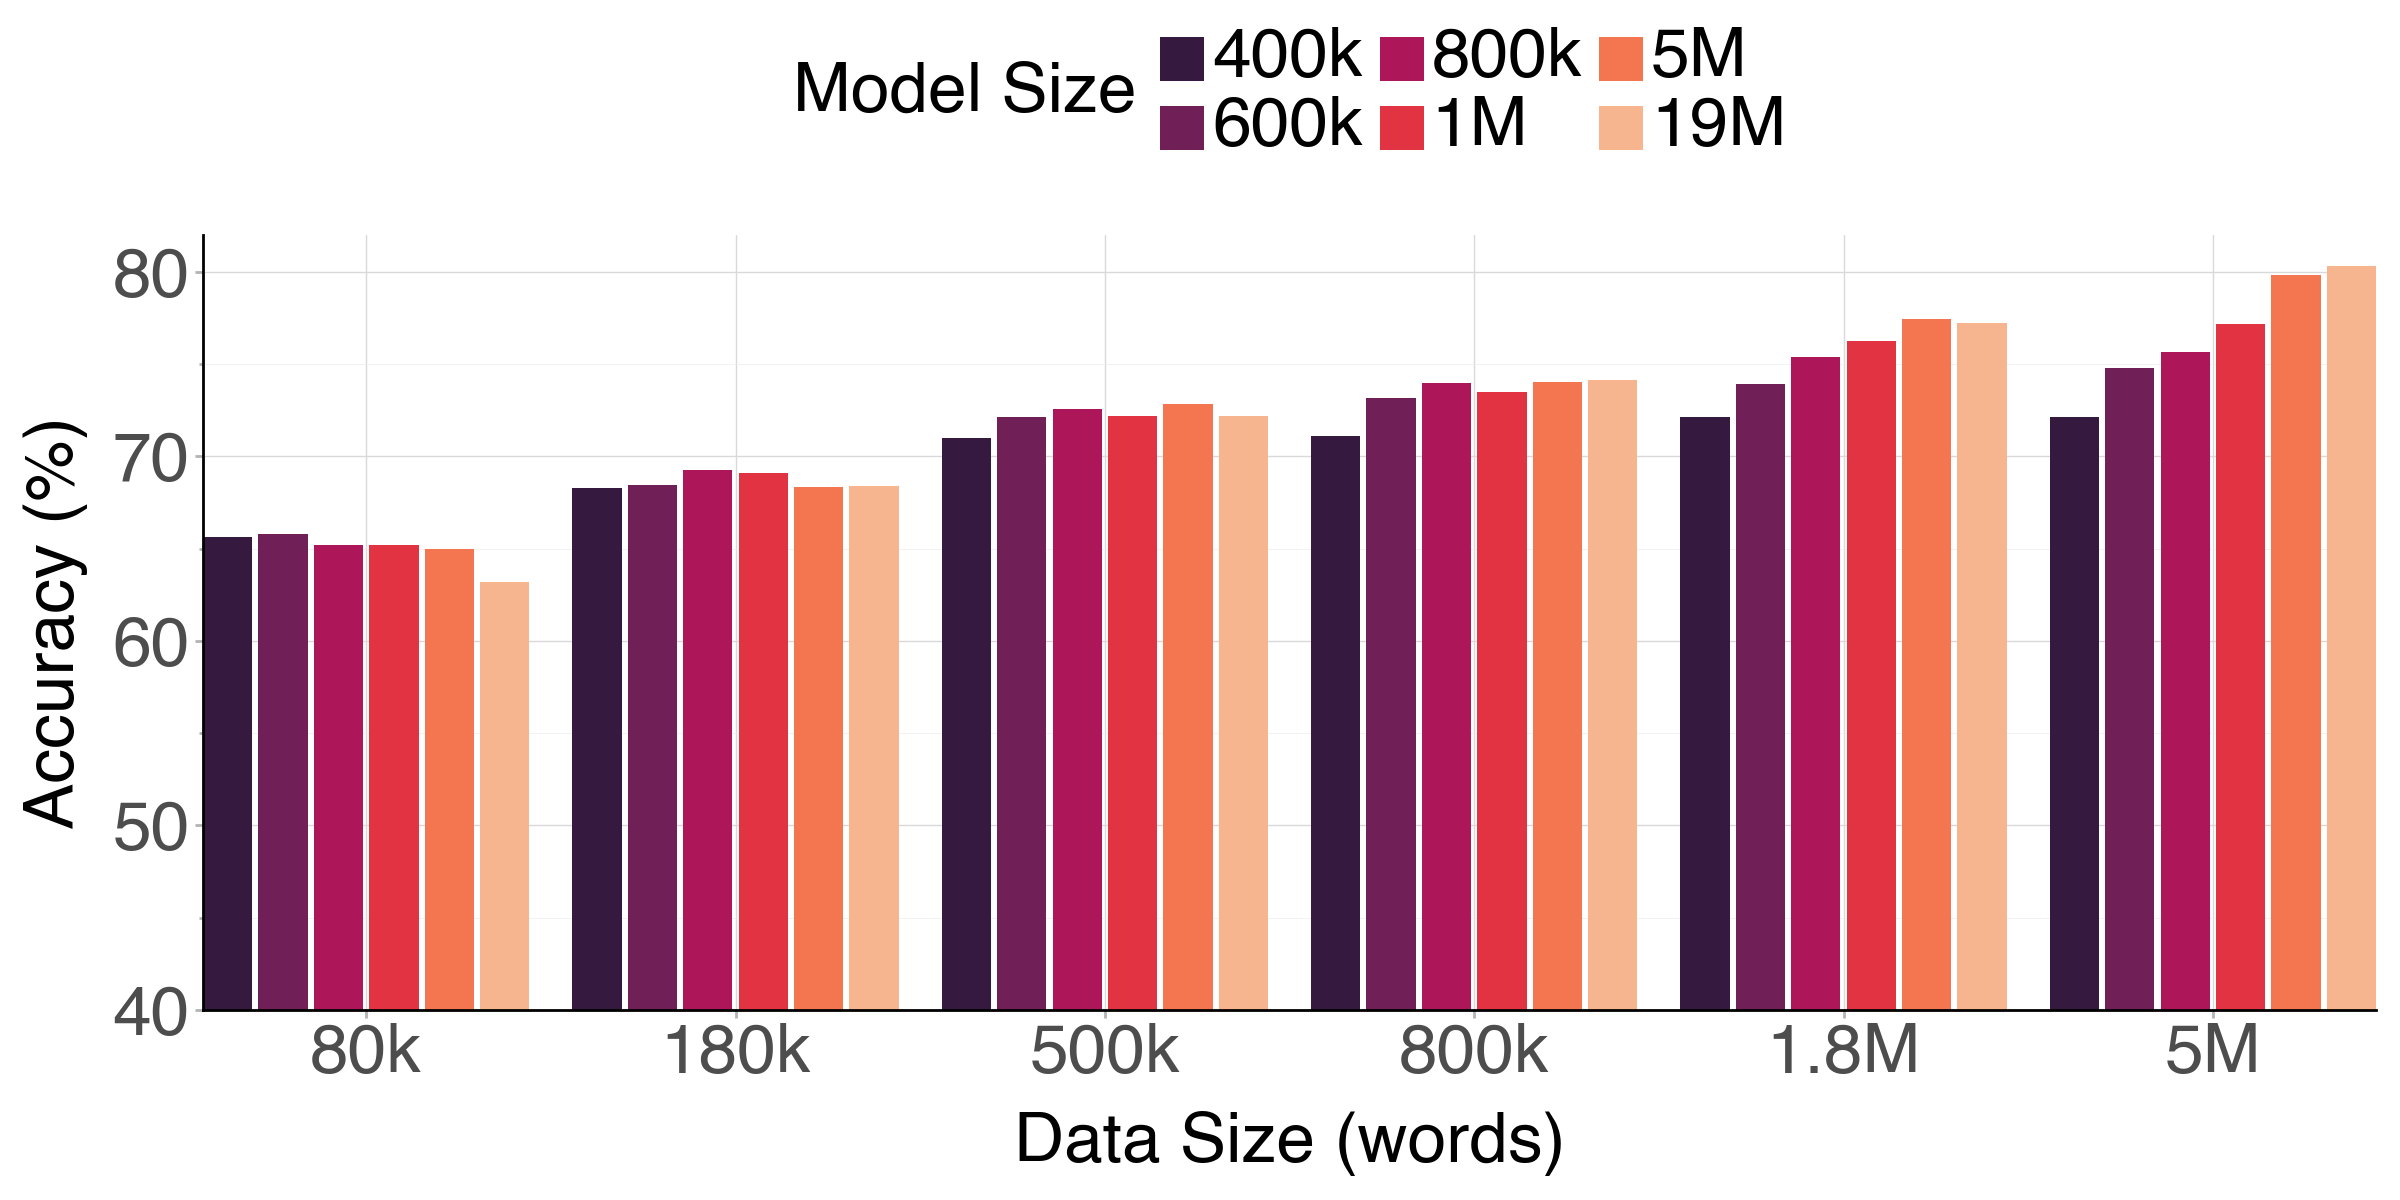
\includegraphics[width=\linewidth]{14Modelling/lexical.png}
    \end{subfigure}
    \hfill
    \begin{subfigure}{0.45\linewidth}
        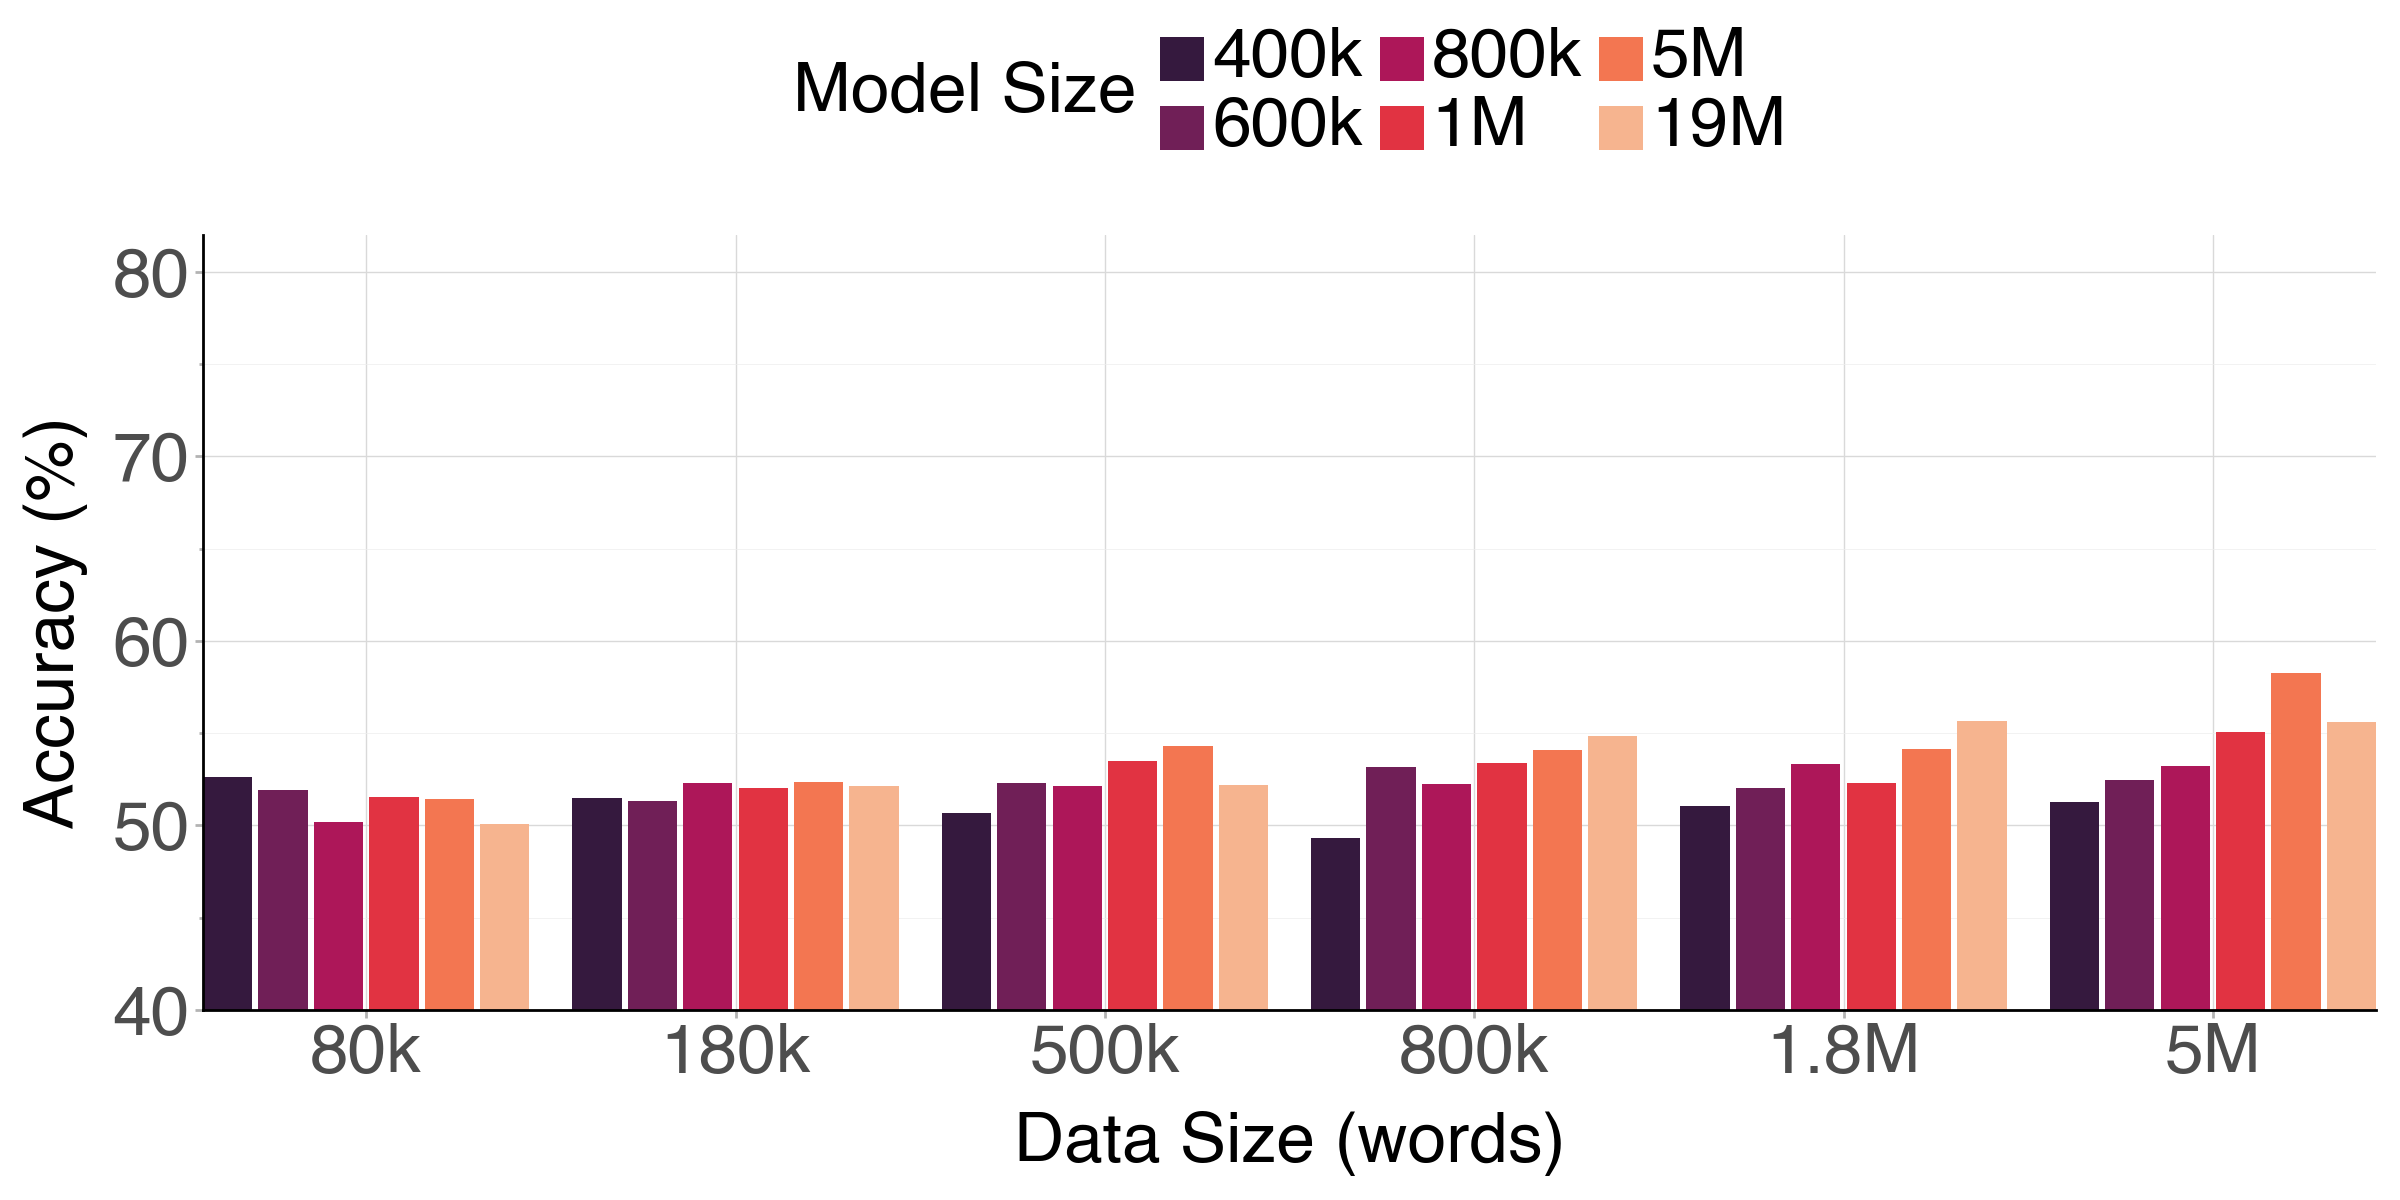
\includegraphics[width=\linewidth]{14Modelling/syntactic.png}
    \end{subfigure}
    \hfill
    \caption{BabySLM lexical score (left) and syntactic score (right) achieved by \gpt trained on the EnglishNA portion of \ipachildes across model sizes and subsample sizes.}
    \label{fig:babyslm}
\end{figure}

\begin{table}[t!]
    \centering
    \small
    \begin{tabular}{c|ccc|ccc}
    \toprule
         Data Size& \multicolumn{3}{c|}{BabySLM Lexical} & \multicolumn{3}{c}{BabySLM Syntactic} \\
         (words) & Model Size & Dropout & Score & Model Size & Dropout & Score \\
         \midrule
         80k & 600k & 0.3 & 65.8 & 400k & 0.5 & 52.6 \\ 
         180k & 800k & 0.3 & 69.3 & 5M & 0.5 & 52.3\\ 
         500k & 5M & 0.3 & 72.9 & 5M & 0.3 & 54.3\\ 
         800k & 19M & 0.5 & 74.2 & 19M & 0.1 & 54.9 \\ 
         1.8M & 5M & 0.3 & 77.4 & 19M & 0.1 & 55.6 \\ 
         5M & 19M & 0.1 & 80.3 & 5M & 0.3 & 58.3 \\ 
    \bottomrule
    \end{tabular}
    \caption{Best model sizes and dropout values for the BabySLM Lexical and Syntactic scores for each subset size of the EnglishNA corpus of \ipachildes.}
    \label{tab:14-bestsizes}
\end{table}

The scaling graphs for the lexical and syntactic scores are given in \cref{fig:babyslm}. For every model size, performance increases with more training data but for a particular data size the largest model is not always the best. For instance, the second smallest model is the best choice for the lexical task if only \q{80}{\thousand} words of data are available, likely due to larger models over-fitting with a sample this small (even with high dropout). The best model parameters for each score and data size are given in \cref{tab:14-bestsizes}, providing a useful reference for what parameters should be chosen when training data is limited.

A comparison between these scores and those of the \q{85}{\million}-parameter model trained reported in \cref{sec:14-babyslm} reveals that phonological knowledge (as measured by the lexical score) requires much less data to acquire than syntactic knowledge. The best model trained on only \q{80}{\thousand} words already achieves a lexical score of \integer{65.8}, improving up to \integer{80.3} for \q{5}{\million} words. Although this increases to \integer{89.6} when a \q{85}{\million}-parameter model is trained on \q{100}{\million} words, this is still far above chance performance of \q{50}{\percent}. By contrast, the syntactic scores at this smaller scale only range from \integer{52.6} for \q{80}{\thousand} words to \integer{58.3} for \q{5}{\million} words, whereas the \q{85}{\million}-parameter model achieves a score of \integer{90.5}. It is also possible that besides requiring more data, phoneme LMs also require more diverse data to learn the syntactic constructions tested. The data from written sources in the BabyLM dataset could be providing an advantage to the large model beyond what is available in child-directed speech.

\section{Discussion}\label{sec:14-discussion}

This chapter set out to establish whether modern language model architectures can encode grammatical knowledge and succeed at language understanding tasks when trained with a phonemic input representations. Overall, \gpt models trained on the BabyLM corpus with a phoneme-based input representation do have decreased performance across standard benchmarks than when trained with the standard subword-based input representation, but this decrease is not substantial. Furthermore, a careful ablation of three transformations that separate the two input representations revealed reasons for this gap in performance. Firstly, using phoneme-level or character-level inputs only leads to a decrease for the GLUE benchmark, despite reduced exposure during training, due to truncation of longer evaluation instances. Secondly, phoneme-based representations lead to a decrease for the BLiMP Supplement tasks because those tasks rely heavily on punctuation, which are not included in phonemic data. Both of these analyses reveal the importance of careful qualitative evaluation of evaluation benchmarks when performing technical experiments with language models. Overall, despite this decrease in performance, it is clear that the \gpt architecture is capable of learning with phoneme-based input representations.

It is not surprising that an alternative input representation would lead to decreased performance, given that the language modelling community has been collectively optimising language model architectures to learn representations for orthographic text, not phonemes, and that the BLiMP and GLUE benchmarks are designed for testing models trained on orthographic text. By contrast, the BabySLM benchmark is specifically designed for smaller models trained on developmentally-plausible corpora across modalities. For this benchmark, the character-level granularity was far more effective than subword-level tokens, and the phonemic modality allows models to be tested for phonological knowledge.

The success of the larger \gpt model on BabySLM indicated that \gpt is a suitable architecture for modelling the utterances in \ipachildes --- supporting phonological experimentation. However, the sections of \ipachildes are much smaller than the BabyLM corpus. To establish the size requirements for phoneme LMs training on much less data, a suite of models were trained on differently-sized subsets of the EnglishNA portion of \ipachildes, indicating that although syntactic generalisation may require more data, phonological knowledge can be learned with as little as \q{80}{\thousand} words. 

% \subsection{The effect of input transformations}

% Another factor to consider is that although we do not change the \gpt architecture or training parameters, the vocabulary size does change, which affects the size of the embedding layer. Character tokenization also leads to reduced exposure to each sentence during training (fewer epochs) because each sentence is represented with more tokens, increasing the number of steps required for each epoch. Furthermore, our initial choice of model parameters may have implicitly favoured the standard orthographic input representation given that the language modelling community has been collectively optimizing these architectures to learn representations for written text, not phonemic streams. Just as the BabyLM challenge seeks to find solutions for low-resource language modelling, we may require an equivalent challenge to identify new methods and architectures for a phonemic input representation. 

% We also found a different pattern for the BabySLM benchmark, that certain transformations increased performance. In some cases, the transformations were even necessary (the lexical measure requiring a model to be trained on phonemic input). Given that the BabySLM benchmark more closely relates to child-language acquisition with its shorter sentences and vocabulary taken from child-directed speech, this result will be of interest to studies using language models to study acquisition.

\section{Summary}

This chapter has explored the effect of training LMs using a phoneme-based input representation, finding that although there is a decrease in performance on standard benchmarks, phoneme LMs are still capable learners which can learn phonological representations even when trained on very little data, suggesting that this paradigm can be successfully used for phonological experimentation. Additionally, the ablation study demonstrated that training LMs with alternative input representations can be used as a diagnostic tool for understanding the how the nature of the input impacts model learning. Specific technical factors revealed through this analysis include the role of punctuation, the role of special tokens and the interaction between sequence length and token granularity.

\Zeb{finish this}

This chapter also established the best parameters to use for different data scales. These parameters are used to train cross-lingual phoneme LMs for phonological experimentation in \cref{chapter:phonology}. Considering alternative combinations of transformations also created novel input representations --- for instance, using \bpe without word boundaries resembles unsupervised word segmentation algorithms. This idea is further explored in \cref{chapter:infotokenisation}, which proposes a novel ...


% Our study explores the effect of training language models using phonemic input representations, which offer both analytical and practical advantages. We develop a pipeline to convert orthographic datasets into a continuous stream of phonemes and leverage this pipeline to train a language model on phoneme streams and evaluate its grammatical and language understanding abilities. Our findings suggest that while phoneme-based input representations result in a slight decrease in model performance on traditional language understanding tasks, it is nonetheless a feasible training paradigm, facilitating future language modelling work, improving phonological interpretability and enhancing speech-based applications.  

%We encourage further research into phonemic input training  to advance our understanding of language models and their applications.

% one of the key advantages of language models—the reliance on orthographic text—and examines how this factor influences their performance. We find that replacing orthographic text with more speech-like representations often leads to a decline in performance across various language understanding tasks and syntactic abilities. Our work highlight the importance of considering data representation in language acquisition research and offers straightforward preprocessing methods as a step toward more human-like input for language models.]
